% !TEX root = ../TechProject.tex

\graphicspath{{Chapter3/}}

\chapter{Machine Learning used for DJing}

\begin{figure}[H]
	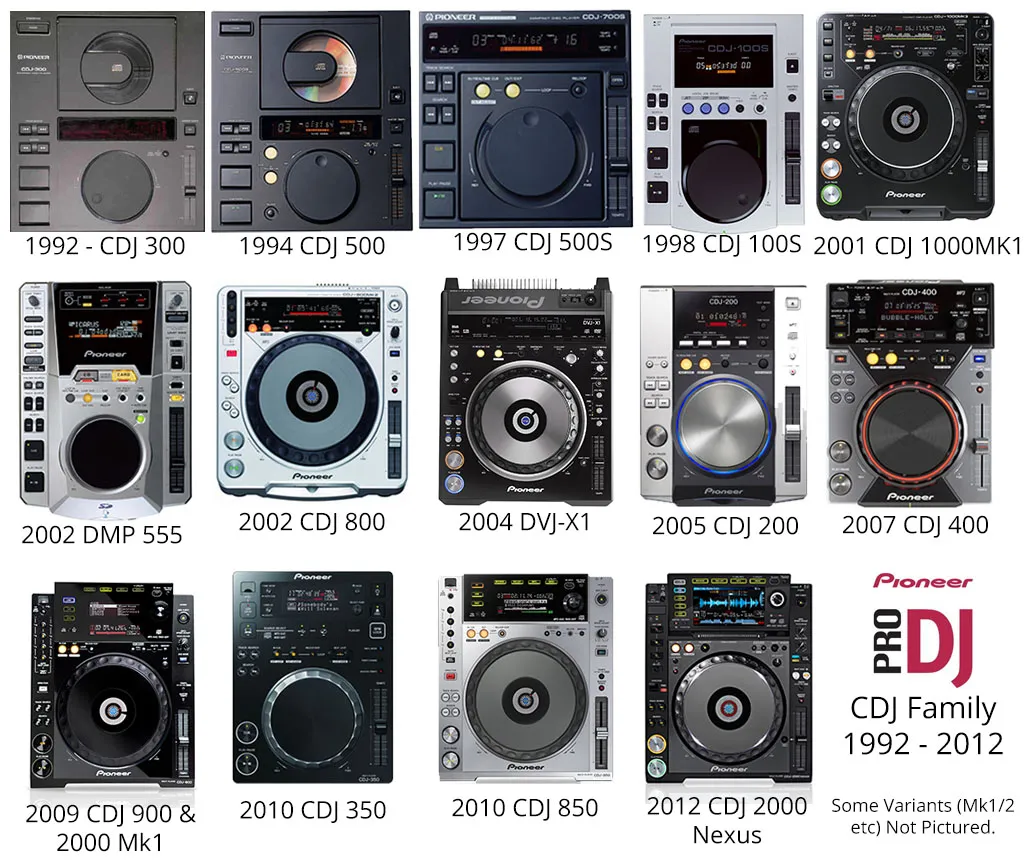
\includegraphics[scale=0.3]{images/pioneers_history}
	\centering
	\caption{Pioneer CDJ models from 1992-2012 \citep{chesters_history_2017}} 
\end{figure}

This chapter answers the following research question:
\\

\textit{Is the proposed method a suitable solution for the automated recommendation of songs suitable for adding to a given DJ set?} 
\\
\\
DJing is a practice that has been the backbone of many sub cultures since the late 60s \citep{brewster_last_2014}. DJing has contributed to the evolution of various genres like Disco, Reggae, and the many forms of electronic dance music \citep{partridge_dub_2010} \citep{reynolds_energy_2013}. DJing traditionally involves two turntables and to transition from one song to another in a stylised or fluid manner. As the rise of digital audio happened within the 1990s saw the creation of CDJs.. CDJs introduced mixing tool softwares such as Pioneers rekordbox. Mixing tool softwares makes use of music information retrival techniques to lower the difficulty of organising and preparing for a DJ set \citep{kim_automatic_2017}. Different implementation of music information retrieval varies from source separation and beat tracking. These tasks involve machine learning and deep learning algorithims, and are now fully embedded in DJ softwares. 

\section{Source Separation}

Source separation is the process of estimating specific sources in one mixed signal. In the context of music, its often used to separate an instrument or voice within a track \citep{sgouros_efficient_2022}. With the recent feats in Deep Learning there has been mass advances in source separation in different fields. One noticable one is the use of U-nets, a convolutional neural network that proved very effective in segmenting biomedical images \citep{ronneberger_u-net_2015}. With the use of spectrograms, a very similar got used in a music source seperation model \citep{jansson_singing_2017}. The following model is then further adapted on the highly popular open source separate made by Deezer called Spleeter \citep{hennequin_spleeter_2020}. Despite no official methods been published, popular DJ manufactor released the Serato Stems update to there DJ software which provides very similar functionality to spleeter but in real time \citep{kirn_review_2023}. This has opened up the possibilities for a DJ to make remixes in real time, separating certain instruments or voices from certain songs.


\section{BPM, key, genre classification}
Briefly touched upon in context based filtering, Audio classification is the building of metadata surrounding a piece of audio by analyzing it \citep{sharma_audio_2021}. As well as proving useful for finding similar songs, audio classification models is used extensively in DJ softwares for calculating tempo, key and other musical attributes.

For key detection, standard machine learning techniques proves powerful enough. The Support Vector Machine proposed by George et. al had an accuracy value of 91.49\% and performed better compared to previous papers \citep{george_development_2022}. Having key information is essential within DJing because assuring the keys either match or modulate functionally assures fluidity in the transition. 

With tempo detection, the current state of the art makes use of Temporal Convolutional Networks to estimate the tempo, as well the up and down beat \citep{bock_deconstruct_2020}. The foundation of the model was explored previously \citep{bock_multi-task_2019}, but found that incorporating an extra dilation rate to each layer of the model gave more accurate results. Knowing the tempo of a given song is one of the main draws of CDJs over vinyl turntables, so further developments in tempo detection will inevitably find itself implemented in DJ software's.

As the case for the BPM and key, the advancement of genre classification has had some significant contirbutions in recent years. The most recent signification is a model that uses short-time fourier transform, pitch, timbre and NMF feautres are extracted from a given piece of audio, which is then fed through a deep belief neural network and a Wale Integreated SnO algorithm \citep{kumaraswamy_optimal_2022}. Advancements in genre classification would be helpful within the DJ world as it would help the organisation of playlists for a given DJ.

\section{Automated Mixing}
As well the advances of classification and separation that will aid a DJ, there are an equal amount of advances that could replace them. In February 2023, Spotify began unravelling its brand new DJ feature, combining situational music recommending accompanied by an AI generated host, mimicking the role of a personal broadcast DJ \citep{naomi_spotify_2023}. Within the research world, there have been advances on not just the mimiking of a human DJ's dialogue, but also the way in which a human would transition from one song to the next.

Spotify have some level of implementation to this already and have ran experiments to show a general further appreciation to playlist if it includes DJ-style transitions \citep{bittner_automatic_2017}. Bittners playlist sequencer also included an attempt of DJ-style tranistions, they used peak detection to determine where abouts in the song the "drops" occurs, and gave specific rules to assure appropriate drop in and drop out points for a given track \citep{bittner_automatic_2017}.  However there means of working out up and down beat was ineffective and greatly effected the fluidity of the transitions. A recent attempt at just the transition aspect of this found that using Boykov-Kolmogorov algorithm alongside spectrogram analysis of the two given songs made for great results for songs with similar tempos and keys \citep{robinson_automated_2023}.

\section{Summary}
\textbf{\textit{Write a summary}}

% note that \Blindocument has 5 numbered levels, despite setting secnumdepth above. I (and many style guides) would suggest using no more than 3 numbered levels (incl. the chapter), with the option of a fourth unnumbered level.